\section{Results}
\subsection{Elastic Scattering}
\RanComment{ A benchmark region of interest is defined between the upper and lower thresholds in cS1 for each channel. This region
is bounded in y space from above by the $^{241}$AmBe NR mean line and below by the lower 3$\sigma$ quantile of the AmBe neutron calibration data. The expected background in the region is $1.7 \pm 0.3$ (lowE) and $1.41 \pm 0.28$ (highE). The number of DM candidates recorded in this region is 1 (lowE), and 0 (highE). }
sout{A total of 50 events are recorded in the signal region distributed in the bins as defined in Table~\ref{table:BinDef}.} The data is compatible with background only hypothesis and no excess is found. For all operators and masses in the range of 10 Gev/$c^2$ to 1TeV$c^2$, \Xehund\ sets the strongest limits on the effective coupling constant $c_i$. These limits are shown in Fig.~\ref{fig:elasticLimit} in black, along with the limits from CDMS-II Si, CDMS-II Ge and SuperCDMS~\cite{CDMSEFT}. For operators 3 and 8, a full CDMS limit is presented, for all other operators only the limit for a 10 GeV/$c^2$ and 300 GeV/$c^2$ are published.  

\begin{figure*}
\begin{minipage}{1.\linewidth}{}
\centerline{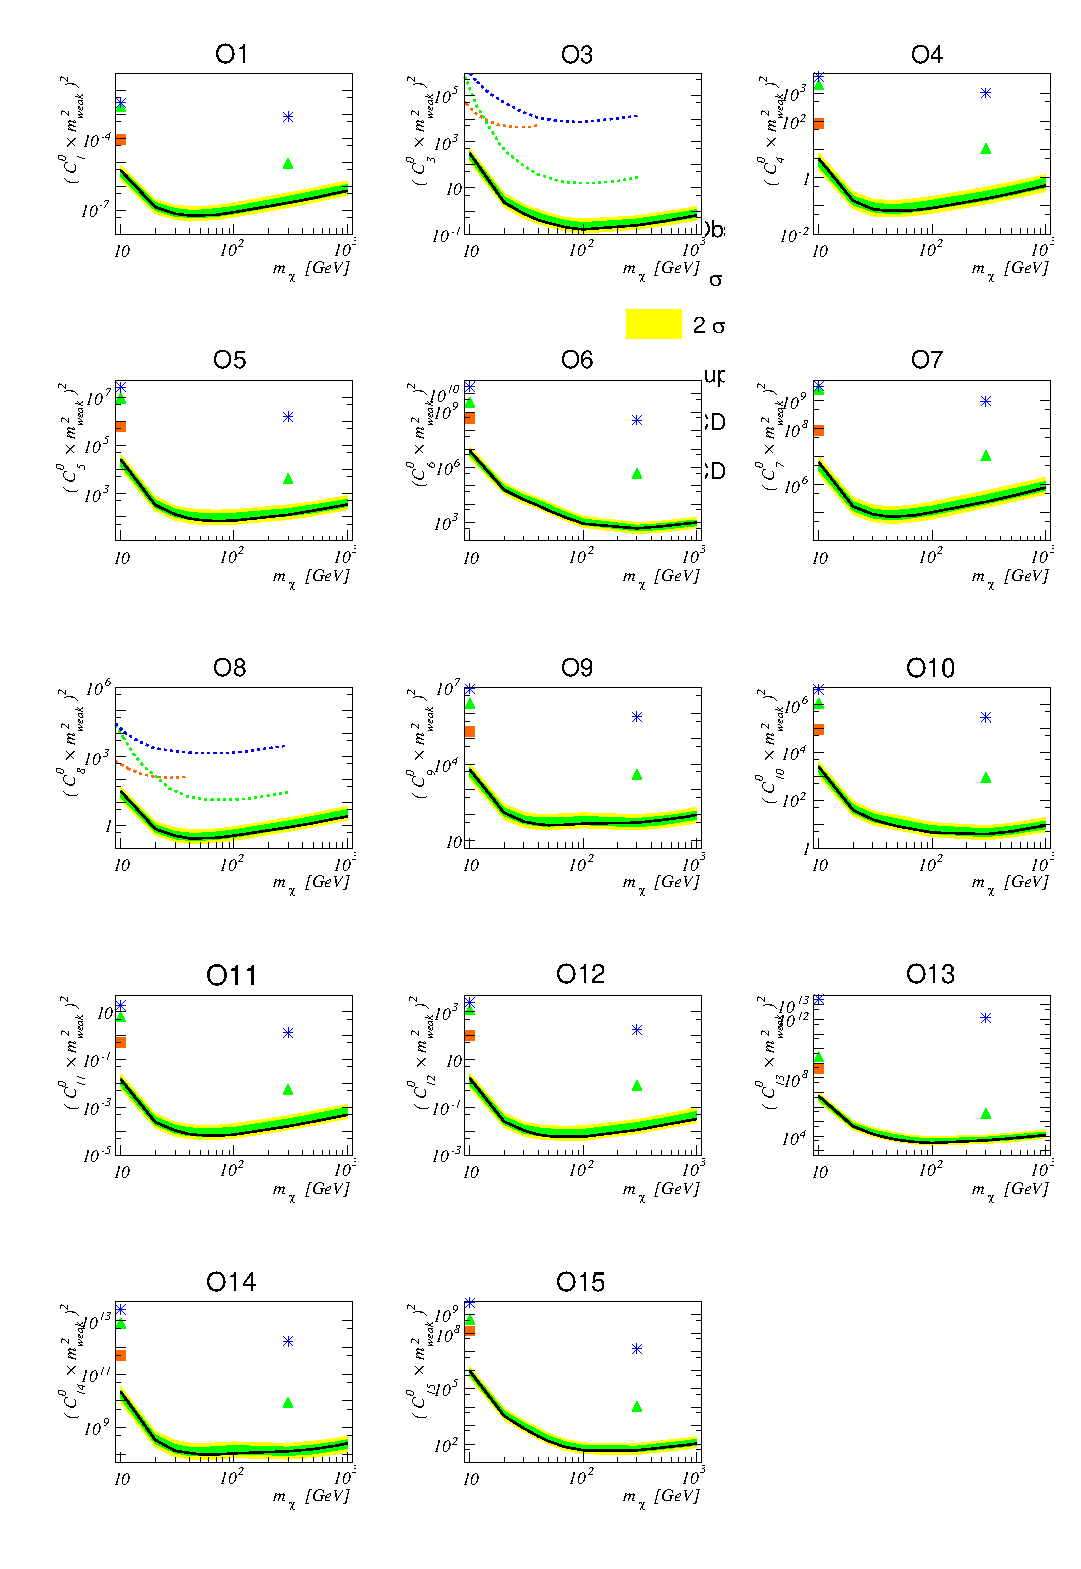
\includegraphics[width=\textwidth,height=\textheight,keepaspectratio]{Figures/SizeTestCDMS.eps}}
%{Figures/ElasticAllLimitCDMS.eps}}
\end{minipage}
\caption{The \Xehund\ limits (90\% CL) Limits on isoscalar dimensionless coupling for all elastic scattering EFT operators are indicated in solid black. The expected sensitivity obtained assuming background only are is shown in green and yellow(1$\sigma$ and 2$\sigma$ respectively). Limits from CDMS-II Si CDMS-II Ge and SuperCDMS cite{CDMS} are presented in blue Astrix ,green triangle and orange rectangle (color online). For operator 3 and 8 a full limit from CDMS is published and indicated by a dashed line in the respected colors.}
\label{fig:elasticLimit}
\end{figure*}


\subsection{Inelastic Scattering}
The limit of inelastic scattering for the SI case ($\mathcal{O}_1$) is shown both as a function of mass splitting and WIMP mass in Fig.~\ref{fig:O1Inel}. Each line represents the 90\% CL for a specific coupling constant value. 

The limits for all other operators are calculated for a WIMP mass of 1 TeV/$c^2$ as a function of the mass splitting $\delta_m$ (Fig.~\ref{fig:InelasticLimit}) 
\begin{figure}[h!]
\centerline{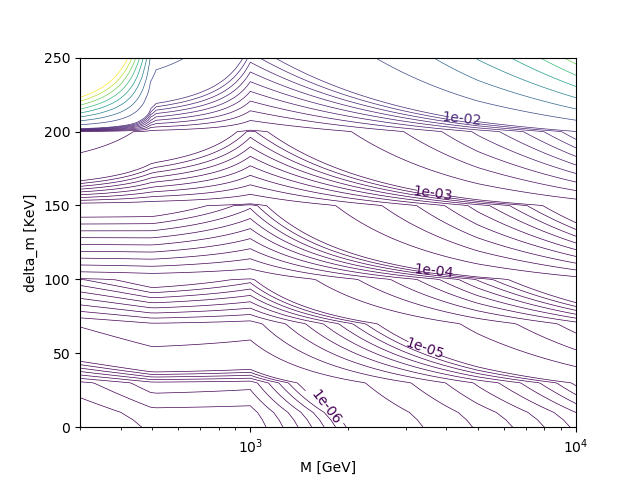
\includegraphics[width=1.\linewidth]{Figures/inelastic_delta_vs_m.png}}
\caption{90\% confidence level limits on coupling constant for $\mathcal{O}_1$ reported as a function of the WIMP mass and mass splitting $\delta$.}
\label{fig:O1Inel}
\end{figure}  



\begin{figure*}
\begin{minipage}{1.\linewidth}
\centerline{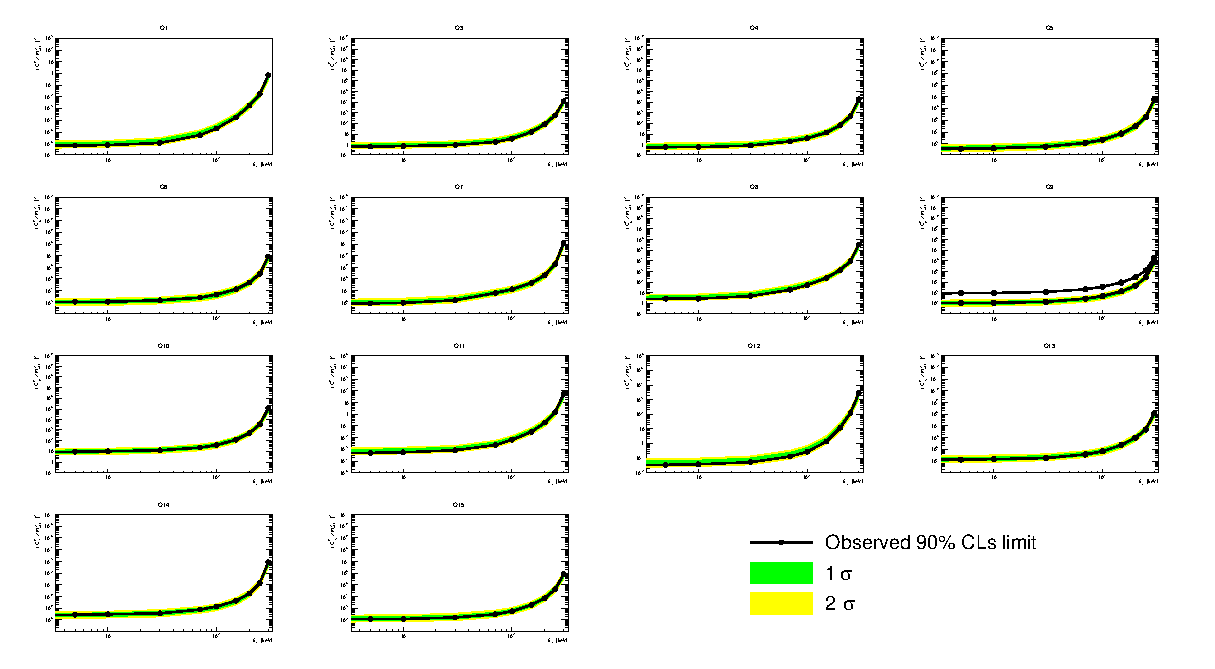
\includegraphics[width=\textwidth,height=\textheight,keepaspectratio]{Figures/FinalInelastic.eps}}
\end{minipage}
\caption{The \Xehund\ limits (90\% CL) Limits on a 1 TeV/$c^2$ WIMP isoscalar dimensionless coupling for all inelastic scattering EFT operators are indicated in solid black. The expected sensitivity obtained assuming background only are is shown in green and yellow(1$\sigma$ and 2$\sigma$ respectively). }
\label{fig:InelasticLimit}
\end{figure*}

\FloatBarrier

